\scanpage{89}
% archive foliation: 91
\figure{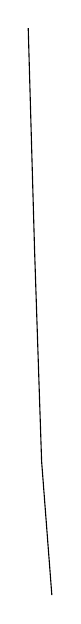
\begin{tikzpicture}\draw (0,0)--(.08,-2.8)--(.17,-5.5)--(.3,-7.2);\end{tikzpicture}}
\uline{Théorème} Soit $k$ un corps alg. clos de car. $\ne2$,
\deleted{Soit $I$ un ens de card $4$, d'où $J$ de card. $3$ et $V=V(J)$. Considérons}

Considérons le groupoïde des $(X,I\hookrightarrow X)$, où $X$ est
une droite projective sur $k$, \deleted{\unsure{tel}}\inserted{$I$ de card $4$}.
Ce groupoïde est équivalent à celui des couples $(I,\zeta\in Z(J(I))^*)$,
en associant à ce couple
\[
X=X(I)\wedge_{\underbrace{V(J(I))}_{\text{ou }V(I)}}t(\zeta,I).
\]
\margin{où $t(\zeta,I)$ est le $V(I)$-torseur $I\wedge X(I)_\zeta^{-1}$}
$I\hookrightarrow X$ est la fibre \inserted{$X_\zeta$} de $X$ en $\zeta$, compte tenu que
\[
\begin{gathered}
X/V(I)\simeq X(I)/V(I)\simeq\unsure{Z|X}(J)\\
X_\zeta\simeq X(I)_\zeta\wedge t(\zeta,I).
\end{gathered}
\]

(\deleted{\unsure{Si}} si $I$ est muni d'un pt $i_0$, on a une description
de $X$ comme $X(I)\wedge_{V(I)}X(I)_\zeta^{-1}$ ; c'est isom. à $X(I)$ une
fois choisi un \unsure{sommet|élément} de $X(I)$ au dessus de $\zeta$.

De façon plus générale, \deleted{\unsure{donc}} la donnée d'un
isom. ``admissible'' $X\simeq X(I)$ équivaut à celle d'un
$V$-isom $I\simeq\deleted{\unsure{Y}}X(I)_\zeta$.
